% Setup - do not change
\documentclass[11pt]{article}
\usepackage[top=0.9in, left=0.9in, bottom=0.9in, right=0.9in]{geometry} 
\usepackage{parskip}

\usepackage[english]{babel}
\usepackage[utf8]{inputenc}
\usepackage{amsmath,amsthm,amssymb,graphicx,pdfpages,lipsum,hyperref}
\usepackage[none]{hyphenat}
\usepackage{csquotes}
\usepackage{hyperref}
\usepackage{multicol}
\usepackage{subfig}
\usepackage{array}
\usepackage{enumitem}  

\renewcommand{\arraystretch}{1.2}

\setlength\parindent{0pt}
%%%%%%%%%%%%%%%%%%%%%%%%%%%%%%%%%%%%%%%%%%%%%%%%%%%%%%%%%%%%%%%%%%%
% add other packages here if required

%% Bibliography are specified in this file. You can also choose inline bib style if you want to. But make sure your citation style is consistent (and proper)
% For more details on citation: https://library.unimelb.edu.au/recite
\usepackage[sorting = none]{biblatex}
\addbibresource{references.bib}

%%%%%%%%%%%%%%%%%%%%%%%%%%%%%%%%%%%%%%%%%%%%%%%%%%%%%%%%%%%%%%%%%%% the '%' symbol denotes comments

% Begin document creation
% DELETE THE \lipsum PLACEHOLDERS WHEN YOU BEGIN
\title{\textbf{Quantitative Analysis of Rideshare Services in Post-Covid Manhattan}
}

\author{
Yi Xiang Chee \\
Student ID: 1165917 \\
%% Replace the link with your github repo
% 1. Remember to escape underscore (\_) in the link.
% 2. Remember to include the commit you want to submit in the link
\href{https://github.com/MAST30034-Applied-Data-Science/mast30034-project-1-yixiangchee/commit/ef32a216a4460b503df59cc0e2c7d75442de66cc}{Github repo with commit}
}

\begin{document}
\maketitle

\section{Introduction}

On April 29 2021, Mayor Bill de Blasio announced the reopening of New York City on July 1, when the city begins its first phase of recovery from the Covid-19 pandemic \cite{nycrecovery}. As the city bounces back from the pandemic, residents started moving back in and driving up rent. At the same time, rideshare services like Uber and Lyft recorded price jumps of 50\% or more, because there are not enough drivers to meet the rebounding demand \cite{pricesurge}.

This report analyzes the recovery of NYC, through the lens of the relationship between \textbf{ridesharing and rental activity} in Manhattan. Two models (Random Forest Regression and Ordinary Least Squares Regression) were studied to forecast pickups in Manhattan neighbourhoods using rent as an indicator. This is established from the perspective of a rideshare company that would like to forecast and match demands, as well as expand accessibility of its services post-pandemic.

\subsection{Dataset}

Our main dataset was the trip record data published by the NYC Taxi and Limousine Commission (TLC) \cite{tripdata}. Specifically, trip data in Manhattan for High-Volume For-Hire Services (HVFHS) was extracted for the year 2021, since our area of interest is ridesharing services (like Uber, Lyft) in a recovering NYC. We will be focusing on the borough of Manhattan, the center of business and social activity in the city, due to limited computing storage. There are about 47 million relevant records; the trip datetime, provider, and pickup location were used and aggregated into total pickups by hour as features (detailed in Section \hyperlink{subsection.2.3}{2.3}).

In conjunction with the trip record dataset, the rental data of Manhattan neighbourhoods in 2021 (published by real-estate platform StreetEasy) was also utilised \cite{rentaldata}. We aim to investigate the co-movement of rental and ridesharing activity, as well as how rent affects pickups in different neighbourhoods, in a city where 70\% of units are renter-occupied \cite{renter}. The monthly median asking rent \footnote{Median was used instead of average to avoid being skewed by extremely expensive rentals.} of each Manhattan neighbourhood were extracted as features.

% use \textbf{} for bold text and \textit{} for italic. 
% \texttt{} creates code blocks akin to `code ticks` in markdown

% Example here used biblatex to manage citations: https://www.overleaf.com/learn/latex/Bibliography_management_with_biblatex , You are free to choose your own way for managing references if biblatex seems too hard.

\section{Preprocessing}

\subsection{Data Linkage}

To use trip data with rental data, data linkage was performed to match taxi zone with neighbourhood. Zones with the same name as their neighbourhood were automatically joined, but some 50 zones required manual linking, where a zone was matched to its closest neighbourhood based on the map provided by both sources \cite{tripdata, rentaldata}. Some taxi zones were excluded from the analysis:
\begin{itemize}
\item Governor's Island/Ellis Island/Liberty Island (no rental property)
\item Randalls Island (no rental property)
\item Central Park (no rental property)
\item Marble Hill (rent unavailable for some months)
\end{itemize}

\subsection{Outlier Detection}
Upon examining the data, $\approx$ 9 million invalid records were removed:  
 
\begin{itemize}
\item \textbf{Trips with dropoff time before pickup}
\end{itemize}
\begin{itemize}
\item \textbf{Trips outside the year of 2021}. Trips that spanned from the end of 2021 to early 2022 were removed as we focused on trips that start and end in 2021.
\item \textbf{Trips with non-zero airport fees}.  Airport fees should be zero for any trips that start and end in Manhattan, which does not have any airports.
\item \textbf{Trips with negative base passenger fare and driver pay}
\item \textbf{Trips with extremely high average speed}. Assuming most drivers drive under the speed limit of 50 mph in Manhattan \cite{speedlimit}, it is safe to remove impossible instances greater than 120 mph, which is unlikely for commercial vehicles \cite{carlimit}.
\end{itemize}

\subsection{Feature Selection and Aggregation}

As Random Forest has a built-in feature selection element, it is less imperative to remove attributes. But for OLS regression, the removal of irrelevant attributes is desirable to alleviate multicollinearity and increase interpretability. Features like tax, tolls, and tips were removed as they are not highly related to analysing or forecasting pickups. The following features were generated and used; they are assumed to be predictive of pickups.

\begin{multicols}{3}
\begin{itemize}
    \item Month
    \item Day of Month
    \item Day of Week
    \item Hour
    \item Pick-up Location ID
    \item HVFHS License Number
    \item Rent of Pick-up Location
\end{itemize}
\end{multicols}

Monthly pickups of all companies and monthly average median asking rent were aggregated for analysis, while hourly pickups of each company (by HVFHS License Number)  in each zone were aggregated for modelling and forecasting.

\section{Exploratory Data Analysis}

\begin{table}[!htb]
\begin{minipage}{.5\linewidth}
    \centering
    \medskip

\caption{Top 5 zones by pickups in 2021} \label{tab:first_table}
\begin{tabular}{|l |c|c| } 
  \hline
    Zone & Pickups \\
    \hline
    East Village & 1438562 \\
    TriBeCa/Civic Center & 1120842 \\
    Union Sq & 1113165 \\
    East Chelsea & 1082294 \\
    West Village & 1068055 \\
  \hline

\end{tabular}
\end{minipage}\hfill
\begin{minipage}{.5\linewidth}
    \centering
    \medskip

\caption{Top 5 zones by rent in 2021}\label{tab:second_table}
\begin{tabular}{|l |c|c| } 
  \hline
    Zone & Avg.Median Rent \\
    \hline
    Midtown North &	7588 \\
    TriBeCa/Civic Center & 6803 \\
    Hudson Sq &	5080 \\
    SoHo &	5080 \\
    Union Sq &	4901 \\
  \hline
\end{tabular}
\end{minipage}
\end{table}

\begin{figure}[h]%
    \centering
    \subfloat[\centering Pickup Frequency by Zone (5\% sample) ]{{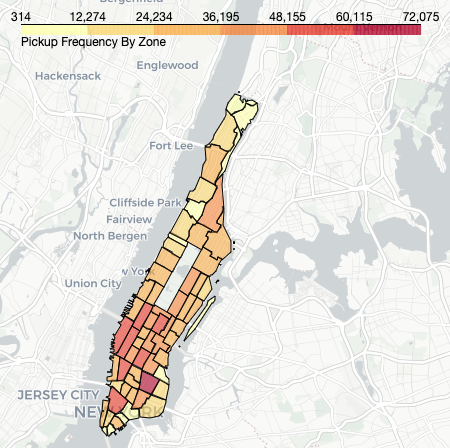
\includegraphics[width=0.45\textwidth]{plots/pickup_map.png} }
    \label{fig:1a}
    }%
    \qquad
    \subfloat[\centering Average Median Rent by Zone (Log-scaled) ]{{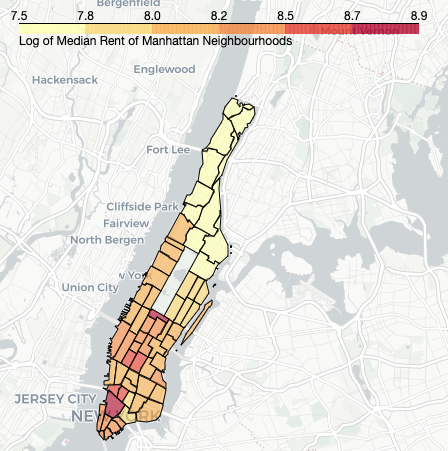
\includegraphics[width=0.45\textwidth]{plots/rent_map.png} }    \label{fig:1b}}%

    \caption{Pickups and Rent in Manhattan in 2021 (Geospatial Plot) }

\end{figure}



\subsection{Pickups\footnote{Random sampling was done only for visualisation purposes (and made sure to accurately reflect population), while analysis and modelling use full distribution.}}
From Table \ref{tab:first_table}, East Village has the highest pickups in 2021 of 1.4 million, which is slightly higher than the next few highest zones in the range of 1-1.1 million. One possible explanation for this is that East Village has a high concentration of university students (NYU), who frequently use rideshare services. As there were no NULL values in our trip record after preprocessing, no imputation was needed. It is also worth noting that there were no records of license \textit{HV0002 (Juno)} present because Juno ceased operations in 2019\cite{juno}. 

\subsection{Rent}
From Table \ref{tab:second_table}, Midtown North has the highest average median rent in 2021. It is located in the Central Park South neighbourhood, which houses some of the most expensive properties in the city. The steep decrease in rent for the next few zones suggests the disparity in rent between taxi zones. Marble Hill was the only zone that had NULL rent data for certain months in 2021. Since it is also located outside of the main Manhattan Island, exclusion of this neighbourhood was justified, hence no imputation was needed as well.
\begin{figure}[h]
    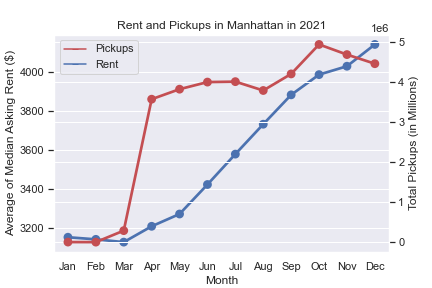
\includegraphics[width=0.7\textwidth]{plots/rent_pickups.png}
    \centering
    \caption{Pickups and Rent in Manhattan in 2021 (Time Series)}
    \label{fig:2}
\end{figure}

\subsection{Relationship between Pickups and Rent}

Two time points of interest are late April (when the reopening was announced) and late June - early July (when the city gradually opened up). In Fig.\ref{fig:2}, rideshare pickups recorded a spike in April and increased steadily until July. Meanwhile, in April, average median rent went from stagnant to steadily increasing for the rest of the year.  In short, rent and pickups exhibit noticeable co-movement, suggesting that residents moving back into the city has an effect on both rent and rideshare demand. 

An interesting area that should be further studied is the difference in increasing patterns for pickups and rent from April - July, namely the April spike in pickups compared to the steady increase in rent. After further investigation, the state of New York expanded Covid vaccine eligibility (from 30 and above to 16 and above) on April 6, hence the spike could be a result of residents using rideshare services to attend their vaccination appointments \cite{cuomo}.

Figure \ref{fig:1a} and \ref{fig:1b} also show that zones with higher rent coincide with higher pickup frequency, as neighbourhoods in lower Manhattan have higher rent and more pickup than upper Manhattan. Indeed, \textit{TriBeCa/Civic Center} and \textit{Union Sq} are amongst the top zones in both Table \ref{tab:first_table} and \ref{tab:second_table}.
\begin{table}[!htb]
\begin{minipage}[b]{.45\linewidth}
    To test the relationship formally, ANOVA was performed on hourly pickups using pickup location and rent as predictors. It is evident in Table \ref{tab:3} that rent is still strongly a significant predictor (p-value extremely small), even in the presence of pickup location.
\end{minipage}\hfill
\begin{minipage}[b]{.5\linewidth}
    \raggedleft
    \medskip

    \caption{ANOVA of Rent in the Presence of Pickup Zone} \label{tab:3}
    \begin{tabular}{ l c c c c c } 
      \hline
      &SS  & DF  & F  &P($>$F) \\
        \hline
        Pickup Zone & 7.28e+08 & 62 & 2510 & 0 \\
        Rent & 3.80e+07 & 1 & 8122 & 0 \\
      \hline
    Residual & 1.95e+09 & 415752 & & \\
     \hline
    \end{tabular}
\end{minipage}
\end{table}

\section{Modelling}
As we have found that rent is a potential indicator for pickup demand in the previous section, we conduct modelling to further investigate this relationship. The two models (Random Forest and OLS) mentioned below take in all attributes listed in Section \hyperlink{subsection.2.3}{2.3} and output a company's pickup numbers given a specific day, hour, and taxi zone. We will be using regression models to do so because our target variable hourly pickup is numerical. Some attributes were one-hot encoded as they are categorical (Pickup Location ID and Company/License Number), or to provide greater flexibility for the linear model to compare between subgroups (Hour and Day).

To evaluate the models, we use trip records ($\approx$ 5 million instances) for the month of April 2022 for prediction. For easy comparison between models, the Root Mean Square Error (RMSE) was chosen as our metric, as it is the preferred evaluation metric for forecasting problems. RMSE indicates the average prediction error of the models.

\subsection{Training and Evaluation}
\textbf{Random Forest}: The regression version, Random Forest Regressor was used \cite{rf}. In contrast to the Classifier, it uses Sum of Squared Errors (SSE) as a splitting metric, and the average of leaf nodes for prediction \cite[263]{dtbook}. The trained Random Forest consists of 20 Random Trees, yielding an RMSE of 58.17 on prediction data. From Table \ref{tab:4}, rent is amongst the top features by feature importance, as calculated using method proposed by Hastie, Tibshirani, and Friedman \cite[368]{ftimp} (more in Section \hyperlink{subsection.4.2}{4.2})

\textbf{Ordinary Least Squares (OLS)}: An ordinary least squares linear regression model was also trained (without regularisation), giving an RMSE of 49.83 on prediction data. The model has an adjusted $R^2$ of 0.5414, meaning that about half of the variation in hourly pickups in training data can be explained by the model. In the model (Table \ref{tab:5}), rent is highly significant (in the presence of other variables). On average, an extra US\$1000 in rent is associated with 7.8 extra hourly pickups. 
\begin{table}[!htb]
    \begin{minipage}[]{.45\linewidth}
    \vspace{16pt}
    \centering
    \caption{Top 3 Features (Random Forest)}
    \label{tab:4}
    \begin{tabular}{ l c } 
      \hline
         Feature & Importance \\
           \hline
        HV0003 (Uber) & 0.56 \\
        HV0005 (Lyft) & 0.15 \\
        Rent & 0.08 \\
        \hline
    \end{tabular}
    \end{minipage}
    \begin{minipage}[]{.45\linewidth}
    \vspace{0pt}

    \caption{Parameter Estimates for Rent (OLS)}
    \label{tab:5}
    \begin{tabular}{ l c c c c } 
      \hline
      & Estimate  & Std.Error  & t  &P($>|t|$) \\
        \hline
        Rent& 7.845e-03 & 1.54e-04 & 50.83 & 0 *** \\
    \hline
    *** $p<0.001$ 
    \end{tabular}
    \end{minipage}
    
\end{table}

Comparing the performances, a conceptually simpler and computationally cheaper algorithm like OLS (with a lower RMSE) performs better than Random Forest, hence is preferred in this scenario.



\subsection{Error Analysis and Discussion}
To look deeper into the behaviour of these models, we perform error analysis on a sample subset of data, using the predictions on April 15 2022 in the taxi zone \textit{Upper West Side North} by both models for Uber (\textit{HV0003}).

From 12am - 7am, both models tend to overestimate pickups; from 8am onwards till late night, they tend to underestimate, except during noon when OLS predicts with high accuracy (Figure \ref{fig:3}). Comparing the predictions made by Random Forest and OLS, it is clear that the predictions by OLS are consistently more accurate than that of Random Forest. OLS gives more dynamic predictions, while Random Forest generates predictions with little to no variation around 60 pickups. 

\begin{figure}[h]
    \makebox[\textwidth][c]{%
    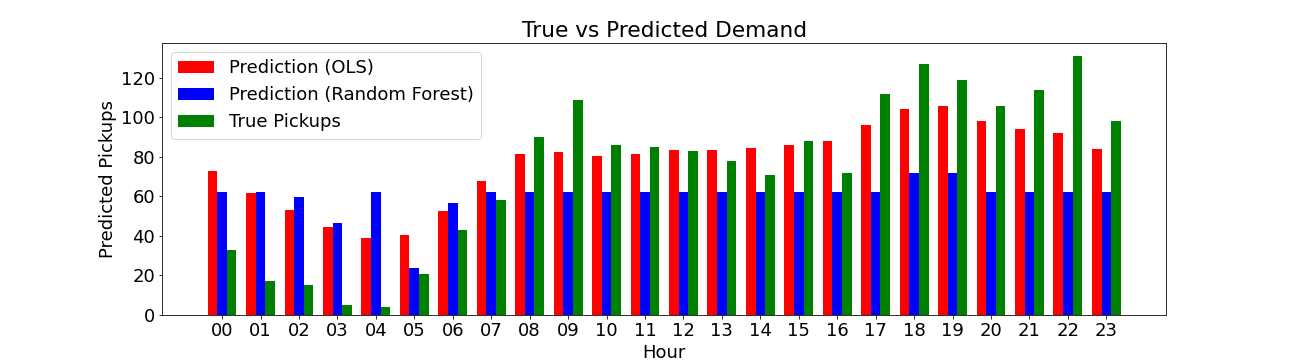
\includegraphics[width=1.24\textwidth]{plots/error_analysis.png}
    }
    \centering
    \caption{Hourly True vs Predicted Pickup Demand (Uber) in Upper West Side North (15th April 2022)}
    \label{fig:3}
\end{figure}

Further examination of the full distribution of the predictions (Figure \ref{fig:4}) shows that predictions made by OLS are smooth and roughly normal, while predictions made by Random Forest are highly concentrated around 3 peaks. This indicates that when regressing using Random Forest, most instances might have always fallen into the same leaf nodes in most Random Trees, giving rather unvarying predictions. Indeed, Table \ref{tab:4} shows that the company variables: \textit{Uber}, \textit{Lyft} (\textit{Via} used as base category) have the largest effect on prediction, hence corresponds to the 3 peaks. There also exist some negative predictions for OLS since it extrapolates, while Random Forest does not.

\begin{figure}[h]%

    \centering
    \subfloat[\centering Random Forest
    ]{{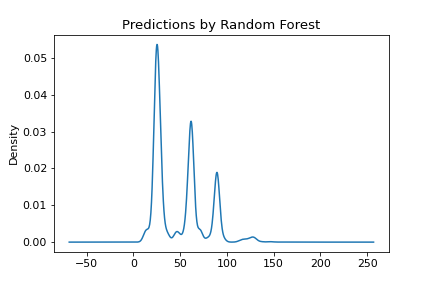
\includegraphics[width=0.45\textwidth]{plots/rf.png} }
    \label{fig:4a}
    }%
    \qquad
    \subfloat[\centering Ordinary Least Squares ]{{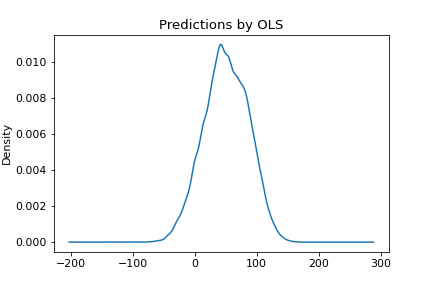
\includegraphics[width=0.45\textwidth]{plots/ols.png} }}%
    \caption{Full April Distribution of Predictions made by Random Forest and OLS}
    \label{fig:4b}%
        \label{fig:4}
\end{figure}

After studying the behaviour of the models, it is apparent that Random Forest is not our preferred model for forecasting, especially in a situation where demands vary dynamically between hours. Moreover, even though OLS has lower RMSE and predicts more accurately than Random Forest, more sophisticated models may be used for even better results, which will be discussed in Section \hyperlink{section.5}{5}.

\section{Recommendations}

As demonstrated in previous sections, rent can be a fairly useful indicator in forecasting rideshare pickups in an area. When used in regression, it is able to predict demand, which is beneficial from the perspective of a rideshare company that is looking to:

\begin{enumerate}[label=(\roman*)]
\item fulfill user demand in all neighbourhoods
\item logistically, ensure there are enough drivers in each neighbourhood to avoid triggering surge pricing (which leads to customer dissatisfaction)
\item anticipate disruptions that future events (e.g. pandemics) might bring on customer demand and/or driver supply
\item understand and outperform rival companies from a competitive standpoint
\item increase app usage and/or driver sign-up in less active areas through localised campaigns (e.g. targeted ads/incentives),
\end{enumerate}
which can all be done by producing and utilising forecasting models as studied above. For instance, combined with the findings in our analysis, we found that upper Manhattan has lower rideshare activity, which is a potential market for companies to expand into.

Moreover, findings from the analysis and model support the argument that there is a disparity in demand between wealthy (or gentrified) and low-income neighbourhoods \cite{politico}. To increase accessibility to transport, rideshare companies could venture into providing cheaper variations of services (e.g. electric scooters, bikes, car pooling), or even working with the city to improve public transport in these areas.

It is also highly recommended that further studies be done incorporating models designated for time series forecasting like Autoregressive Integrated Moving Average (ARIMA) (which regresses on lagged values and moving averages) or Autoregressive Distributed Lag (ARDL) (which incorporates explanatory variables), as these models are better at capturing temporal relationships in data like hourly pickups. Some external data that could be useful to study and include as attributes are the NYC recovery index \cite{nycindex} and public transport data (to study rideshare's interaction with public transportation infrastructures).

\section{Conclusion}
In short, we examined the recovery of Manhattan in 2021 through rideshare and rental activity. From our findings in analysis and modelling, we conclude that the rent of a taxi zone is a significant indicator in predicting rideshare pickups, which can be used by rideshare companies to forecast demand in regression models like Ordinary Least Squares or time series models. We also found that Lower (Downtown) Manhattan (e.g. East Village) has higher demand than Upper (Uptown) Manhattan, as well as higher rent. Subsequently, these findings can be utilised to help a rideshare company understand the market and better inform its operation strategies to increase profitability.



\clearpage

% BEGIN REFERENCES SECTION
\printbibliography

\end{document}